\section{Stabilność procesu uczenia}
\label{sec:wyniki-stabilnosc}

W celu
przedstawienia powtarzalności procesu treningowego obliczyłem dla kolejnych checkpointów
odchylenie standardowe walidacyjnego EV pomiędzy pięcioma seedami
wybranych konfiguracji.

Wyniki przedstawiam na rysunku~\ref{fig:seed-variability-over-training}.
Na osi poziomej znajduje się liczba epizodów treningowych, a na osi
pionowej odchylenie standardowe walidacyjnego EV pomiędzy pięcioma
seedami wybranych konfiguracji DQN i REINFORCE. Krzywa REINFORCE
przez większość treningu leży wyraźnie powyżej krzywej DQN i po
50\,000 epizodach nadal rośnie, podczas gdy zmienność DQN pozostaje
w przybliżeniu na tym samym poziomie.

\begin{figure}[htbp]
    \centering
    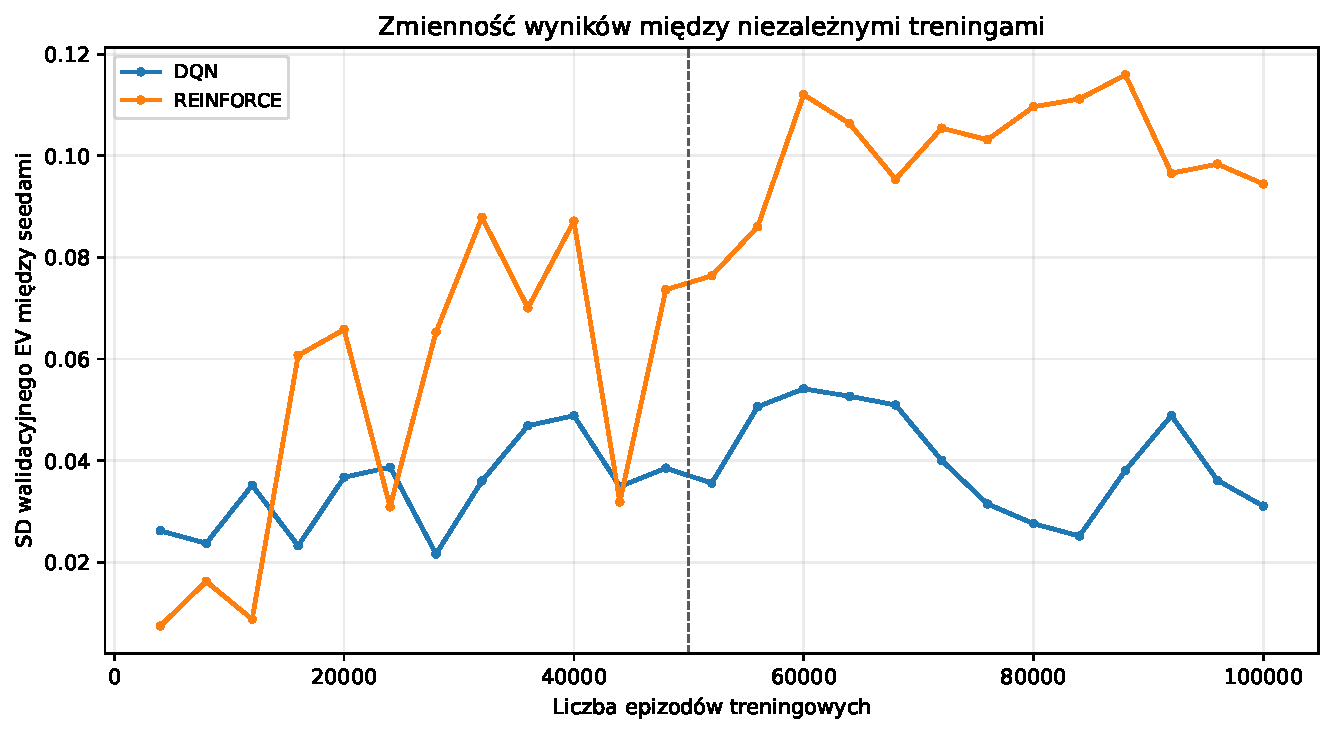
\includegraphics[
        width=0.9\textwidth
    ]{../experiments/results/final_analysis/08_seed_variability_over_training.pdf}
    \caption{Zmienność walidacyjnego EV między seedami podczas
    treningu.}
    \label{fig:seed-variability-over-training}
\end{figure}

DQN utrzymywał relatywnie niewielki rozrzut pomiędzy niezależnymi
przebiegami. REINFORCE wykazywał natomiast okresy znacznie większej
zmienności, co jest zgodne zarówno z krzywymi uczenia, jak i wynikami
końcowej ewaluacji. Oznacza to, że w badanym ustawieniu REINFORCE
częściej prowadził do jakościowo różnych polityk.

Na rysunku~\ref{fig:gradient-norm-reward-scale} porównuję przebieg normy gradientu 
dla obu wariantów funkcji nagrody, dla konfiguracji
wykorzystujących reprezentację FEATURES. Na osi poziomej znajduje się
liczba epizodów treningowych, a na osi pionowej, w skali
logarytmicznej, norma gradientu uśredniona po pięciu seedach, dla DQN
dodatkowo wygładzona oknem 500 epizodów ze względu na aktualizację co
krok środowiska. Norma gradientu dla nagrody skalowanej jest w obu
algorytmach systematycznie niższa niż dla zysku netto, choć różnica
skali jest znacznie większa dla DQN.

\begin{figure}[htbp]
    \centering
    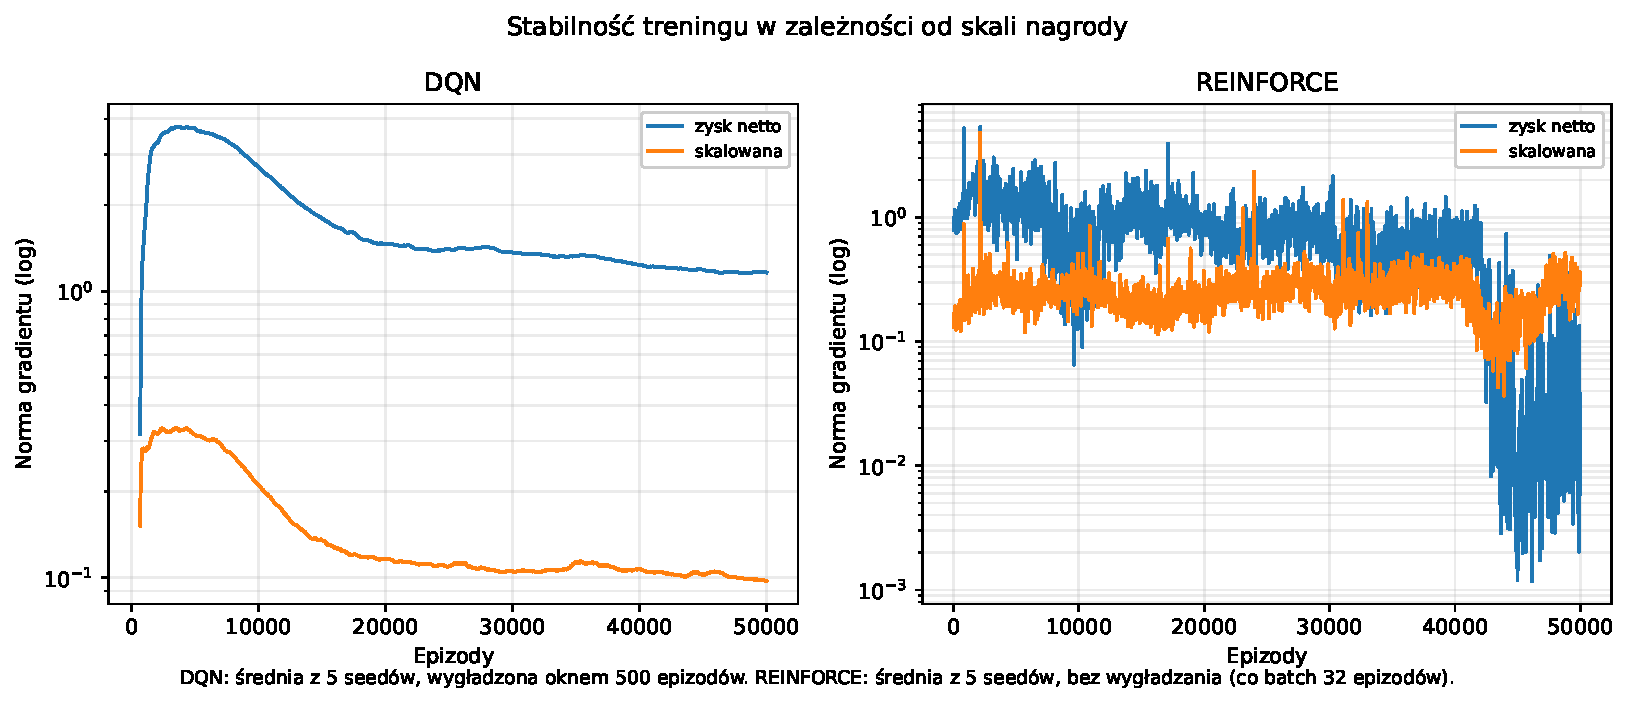
\includegraphics[
        width=\textwidth
    ]{../experiments/results/final_analysis/19_training_stability_by_reward_scale.pdf}
    \caption{Norma gradientu w zależności od skali funkcji nagrody.}
    \label{fig:gradient-norm-reward-scale}
\end{figure}

Skalowanie nagrody wyraźnie zmieniało skalę gradientów powstających
podczas optymalizacji. Nie oznacza to jednak automatycznie poprawy
końcowej jakości polityki. Jak pokazały wyniki z
sekcji~\ref{sec:wyniki-funkcja-nagrody}, mniejsza skala sygnału
optymalizacyjnego nie przekładała się na uniwersalną przewagę
skalowanej funkcji nagrody.

Analiza gradientów pokazuje,
że zmiana funkcji nagrody wpływa na przebieg aktualizacji parametrów,
ale sama kontrola skali gradientu nie rozwiązuje problemów związanych
ze stabilnością uczenia ani nie gwarantuje uzyskania lepszej
strategii.
